\documentclass[tikz,border=4pt]{standalone}
% Shared style for every figure and for the deck: one accent, one
% highlight, thin lines, rounded nodes, nothing decorative.
\usepackage[T1]{fontenc}
\usepackage{lmodern}
\renewcommand{\familydefault}{\sfdefault}
\usepackage{tikz}
\usetikzlibrary{arrows.meta,positioning,calc,shapes.misc,fit,backgrounds,decorations.pathreplacing}
\definecolor{ink}{RGB}{40,40,40}
\definecolor{soft}{RGB}{150,150,150}
\definecolor{faint}{RGB}{225,225,225}
\definecolor{accent}{RGB}{0,95,115}
\definecolor{accentlight}{RGB}{214,232,236}
\definecolor{warn}{RGB}{196,84,40}
\definecolor{warnlight}{RGB}{247,226,216}
\tikzset{
  every picture/.style={color=ink, line width=0.5pt, font=\small},
  node distance=12mm and 18mm,
  box/.style={draw=ink, rounded corners=2pt, fill=white, inner sep=5pt, minimum height=7mm, align=center},
  maker/.style={box, minimum width=18mm},
  cat/.style={box, inner sep=3.5pt, minimum height=6mm},
  root/.style={box, fill=accentlight, draw=accent},
  bad/.style={box, fill=warnlight, draw=warn},
  ghost/.style={box, draw=soft, text=soft, dashed},
  flow/.style={-{Stealth[length=4pt,width=3.5pt]}, line width=0.5pt},
  sub/.style={-{Stealth[length=4pt,width=3.5pt]}, line width=0.5pt, color=soft},
  strong/.style={flow, color=accent, line width=0.8pt},
  wrong/.style={flow, color=warn},
  lbl/.style={font=\footnotesize, text=ink, inner sep=1.5pt, fill=white},
  note/.style={font=\footnotesize, text=soft, align=center},
  rate/.style={font=\footnotesize, text=accent, inner sep=1pt, fill=white},
}

\usepackage{amsmath}
\usepackage{pgfplots}
\pgfplotsset{compat=1.17}

\begin{document}
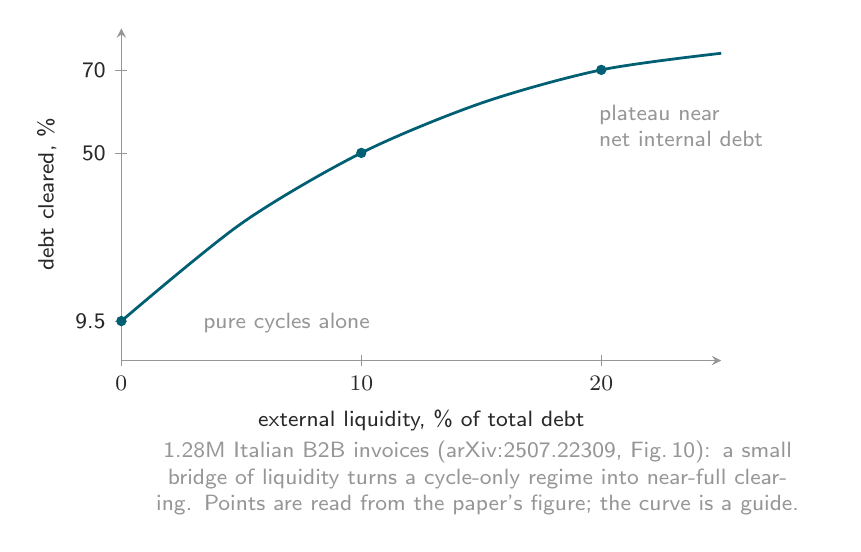
\begin{tikzpicture}
\begin{axis}[width=92mm, height=58mm, axis lines=left, axis line style={soft}, tick style={soft},
  xlabel={external liquidity, \% of total debt}, ylabel={debt cleared, \%},
  xmin=0, xmax=25, ymin=0, ymax=80, xtick={0,10,20}, ytick={9.5,50,70},
  yticklabels={9.5,50,70}, label style={font=\footnotesize, text=ink}, tick label style={font=\footnotesize, text=ink},
  clip=false]
  \addplot[accent, line width=1pt, smooth] coordinates {(0,9.5) (5,33) (10,50) (15,62) (20,70) (25,74)};
  \addplot[only marks, mark=*, mark size=1.6pt, accent] coordinates {(0,9.5) (10,50) (20,70)};
  \node[note, anchor=west, align=left] at (axis cs:3,9) {pure cycles alone};
  \node[note, anchor=north west, align=left] at (axis cs:19.5,64) {plateau near\\ net internal debt};
\end{axis}
\node[note, anchor=north west, text width=88mm] at (0,-9mm) {1.28M Italian B2B invoices (arXiv:2507.22309, Fig.\,10): a small bridge of liquidity turns a cycle-only regime into near-full clearing. Points are read from the paper's figure; the curve is a guide.};
\end{tikzpicture}
\end{document}
